\documentclass[A4, 10pt, conference]{ieeeconf}	

\IEEEoverridecommandlockouts                              
\overrideIEEEmargins
% Autres classes disponibles : report, book, slides
% Options possibles : 	11pt, 12pt (taille de la fonte)
%                     			oneside (recto simple)
%                     			twoside (document recto-verso)
\usepackage{color,graphicx}
\usepackage{psfrag}
\usepackage[english]{babel}
\usepackage{amsmath,amssymb,xfrac}

\topmargin +8pt
\oddsidemargin -25pt
\evensidemargin -25pt

%\usepackage{mathabx}
\usepackage[thref]{ntheorem}
\usepackage{float}
\newcommand{\jo}{(j\omega,\rho)}
%\renewcommand{\IEEEQED}{\IEEEQEDopen}
\renewcommand{\vec}[1]{\mathbf{#1}}
%\DeclareRobustCommand*{\IEEEauthorrefmark}[1]{%
  %\raisebox{0pt}[0pt][0pt]{\textsuperscript{\footnotesize\ensuremath{#1}}}}

\begin{document} 

\title{\LARGE \bf $H_{\infty}$ Smith Predictor Design for Time-Delayed MIMO Systems via Convex Optimization}

\author{Achille Nicoletti$^{1,2}$ and Alireza Karimi$^{1,3}$% <-this % stops a space
\thanks{$^{1}$Automatic Control Laboratory
Ecole Polytechnique F\'{e}d\'{e}rale de Lausanne (EPFL),
1015 Lausanne, Switzerland}%
\thanks{$^{2}$ {\tt\small achille.nicoletti@epfl.ch}}%
\thanks{$^{3}$ {\tt\small alireza.karimi@epfl.ch}}%
}

\maketitle
\thispagestyle{empty}
\pagestyle{empty}

\begin{abstract}
A new method for robust fixed-order $H_{\infty}$ controller design for uncertain time-delayed MIMO systems is presented. It is shown that the $H_{\infty}$ robust performance condition can be represented by a set of convex constraints with respect to the parameters of a linearly parameterized primary controller in the Smith predictor structure. Therefore, the parameters of the primary controller can be obtained by convex optimization. The proposed method will be applied to stable MIMO models with uncertain dead-time and with multimodel and frequency-dependent uncertainty. The performance of this method is illustrated by simulation examples of industrial processes.
\end{abstract}

%\begin{IEEEkeywords}
%Robust controller, convex optimization, H-infinity, transfer function %uncertainty, Smith predictor, MIMO time delay.
%\end{IEEEkeywords}


\section{Introduction}
Many dynamical systems in the industry possess unavoidable time delays. These delays can be caused by accumulation of time lags for dynamic systems interconnected in series, transportation delay or measurement delay \cite{NC07}. Time delays in control loops can cause significant complications in modern industrial applications. The rapid development in data and communication network technologies has caused a need for real-time data processing \cite{LHW08}. The first time-delay compensation method was proposed in the late 1950s by \cite{Smi57}. This method is known as the Smith Predictor (SP), and it has become one of the most widely implemented control schemes used to regulate industrial systems with time delays. 

The SP, however, is somewhat limited in its performance, since an accurate model of the system is generally required for satisfactory operation. In certain circumstances, small modeling errors may lead to undesirable performance, where the system can become unstable. For this reason, research efforts have been focused on robustness issues of the SP. 

\iffalse
\begin{figure}[h]
\centering
\psfrag{rr}{\small $r$}
\psfrag{cc}{\small $C(s)$}
\psfrag{uu}{\small $u$}
\psfrag{pp}{\hspace{-0.15cm}\small $P(s)$}
\psfrag{gn}{\hspace{-0.2cm}\small $G_n(s)$}
\psfrag{ex}{\hspace{-0.2cm}\small $e^{-\tau_n s}$}
\psfrag{yp}{\small $y_p$}
\psfrag{yy}{\small $y$}
\psfrag{pl}{\scriptsize $+$}
\psfrag{mi}{\scriptsize $-$}
\psfrag{dis}{\small $d$}
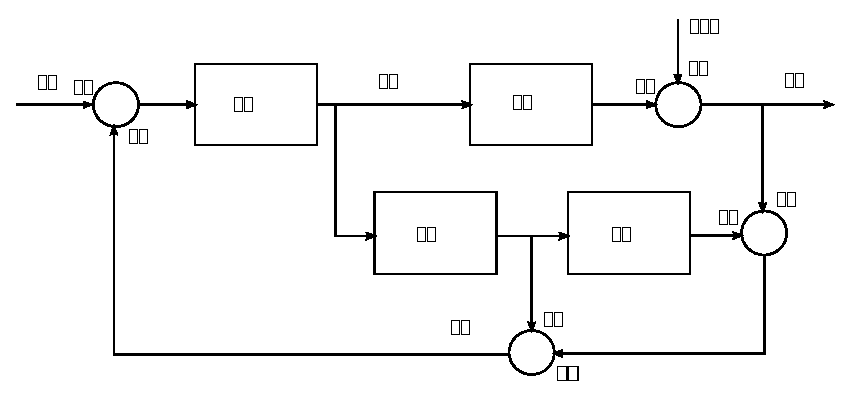
\includegraphics[width=0.8\columnwidth]{pics/SISO_block.eps}
\caption{Smith Predictor}
\label{fig:smith_siso}
\end{figure}%
\fi

Many researchers are interested in the optimal control of dead-time
systems, especially $H_{\infty}$ control, i.e., to find a controller to
internally stabilize the system and to minimize the $H_{\infty}$-norm of an associated transfer
function. Many relevant results have been presented in this framework using 
modified versions of the SP. See, for instance, \cite{Mir03}, \cite{MZ00} and \cite{Zho03a}. Recently, the single-input-single-output (SISO) SP has been extended and generalized for multiple-input-multiple-output (MIMO) systems. In \cite{SBP09}, a structured uncertainty approach was implemented for SP's with diagonal delay matrices. This method, however, does not consider general and distinct time delays for each element of the plant transfer matrix. A diagonal $H_2$ optimal controller for non-square plants is designed by factorization methods in \cite{ZL06}. In \cite{NC00}, a generalized predictive control (GPC) method is implemented on MIMO SP systems with multiple delays.   
These control techniques, although efficient, are quite complex from both the design and implementation perspective.

There are a wide variety of industrial applications that involve MIMO processes with time delays, and it is of practical interest to develop robust control techniques for such systems. The proposed control scheme is based on the ideas presented in \cite{VK13}  for SP design of SISO systems and in \cite{GKL10b} for designing decoupling MIMO controllers. However, in this paper, the SP design method for computing $H_\infty$ controllers for SISO models is extended to MIMO SP's with process plants that possess uncertain time delays. A convex optimization approach is implemented to design a linearly parameterized primary controller in a SP structure for a MIMO system with uncertain time delays. %Due to the number of time delay uncertainties associated with the SISO subsystems of the overall MIMO process, a controller must be designed such that the $H_\infty$ performance criterion is satisfied for each combination of these uncertainties. 

This paper is organized as follows: In Section (\ref{sec:2}), the class of models, controllers and control objectives are defined. Section (\ref{sec:3}) will discuss the control design methodology and stability conditions of the proposed method for the MIMO Smith predictor. This methodology is based on the convex constraints in the Nyquist diagram. Section (\ref{sec:4}) will demonstrate the effectiveness of the proposed method by considering several case studies from industrial processes. Finally the concluding remarks are given in Section (\ref{sec:5}). 
\section{Problem Formulation}
\label{sec:2}
In this section, the SP for MIMO systems with generalized time delays is investigated. For notation purposes, bold face characters will represent transfer function matrices.
\subsection{Class of models}
Let $n_o$ and $n_i$ represent the number of outputs and the number of inputs of a system, respectively. The set of LTI-MIMO stable strictly proper  models with multiplicative uncertainty and  uncertain time delays can be defined as follows: 
\begin{equation}\label{eq:setpmimo}
\mathcal{P}=\{\vec{P}_c(s)[\vec{I}+\Delta_c(s) \vec{W}_{2_{c}}(s)];\hspace{0.5cm} c=1,\ldots,m\}
\end{equation}
where each element in $\vec{P}_c(s)$ possesses a time delay that can vary over a range of specified values, and $\vec{W}_{2_{c}}$ is a transfer function matrix that represents the multiplicative input uncertainty of the system. $\Delta_c(s)$ represents the unknown stable transfer function matrix satisfying $\| \Delta_c \|_{\infty} < 1 $. For simplicity, one model from the set $\mathcal{P}$ will be investigated, and the subscript $c$ will be omitted. The uncertain $n_o \times n_i$ time delayed plant has the following form:
\begin{equation}\label{eq:mimo_p}
\vec{P}(s)=
\begin{bmatrix}
G_{11}(s)e^{-\tau_{11} s} & \cdots & G_{1n_{i}}(s)e^{-\tau_{1n_{i}} s} \\ \vdots & \ddots & \vdots \\ G_{n_{o}1}(s)e^{-\tau_{n_{o}1} s} & \cdots & G_{n_{o}n_{i}}(s)e^{-\tau_{n_{o}n_{i}} s}
\end{bmatrix}
\end{equation}
where $G_{qp}(s)$ is a strictly proper delay-free transfer function, and $\tau_{qp}$ is the uncertain time-delay of the process for $p=1,\ldots, n_i$ and $q=1,\ldots, n_o$. Note that $\tau_{qp}$ is a set that is composed of elements $\tau_{qp_{i}}$ for $i=1,\ldots, l$ and belongs in the domain $\{ \tau_{qp} \in \mathbb{R}:\tau_{qp_{i}} > 0 \ \forall \: \{p,q,i\} \}$.


\subsection{Class of controllers}
As stated in \cite{GKL10b}, an $n_i \times n_o$ matrix can be formed to represent the controller $\vec{C}(s,\rho)$. The elements of $\vec{C}(s,\rho)$ will possess linearly parameterized elements
\begin{equation} \label{eq:mimo_con}
C_{pq}(s,\rho)=\rho^T_{pq}\phi_{pq}(s)
\end{equation}
where $\rho^T_{pq}$ is a vector of parameters, and $\phi_{pq}(s)$ is a vector of stable transfer functions chosen from a set of orthogonal basis functions. The non-diagonal elements of $\vec{C}(s,\rho)$ strive to decouple the system, while the diagonal elements aim to control the single-loop subsystems. The main purpose of parameterizing the controller in this manner is due to the fact that the components of the open loop transfer function can be written as a linear function of the control parameters $\rho$,
\begin{equation}
\rho=[\rho_{11},\ldots,\rho_{1_{n_{i}}},\ldots,\rho_{n_{o}1},\ldots,\rho_{n_{o}n_{i}}]
\end{equation}
\subsection{Design specifications}\label{sec:mimo_des}
Fig. \ref{fig:mimo_block} displays the SP for the MIMO case,
%\footnote{Note that the block diagram for the SP has been reconfigured for the MIMO case. In this manner, the uncertain plant is generalized where each element in (\ref{eq:mimo_p}) can posses a distinct and unique range of time delays.}. 
where $\vec{G}_n(s)$ is an $n_o \times n_i$ nominal delay-free transfer function matrix with elements $G_{qp}(s)$, and $\vec{P}_n(s)$ is an $n_o \times n_i$ nominal transfer function matrix that includes the nominal values of the time delays, which is comprised of elements $G_{qp}(s)e^{-\zeta_{qp}s}$ (where $\zeta_{qp}$ represents the $qp$-th nominal time delay). Both $\vec{Y}(s)$ and $\vec{R}(s)$ are $n_o \times 1$ column vectors that possess elements $y_q(s)$ and $r_q(s)$, respectively. The transfer function from the inputs of $\vec{C}(s)$ to $\vec{Y}_p(s)$ will represent the open-loop transfer function,
\begin{equation}\label{eq:oltfmimo}
\vec{L}(s)=[\vec{P}(s)+\vec{H}(s)]\vec{C}(s)
\end{equation}
where $\vec{H}(s)=\vec{G}_n(s)-\vec{P}_n(s)$. Notice that if $\vec{P}(s)=\vec{P}_n(s)$, then $\vec{L}(s)=\vec{G}_n(s)\vec{C}(s)$. Since the class of controllers to be designed for this system are linearly parameterized, the elements of the controller $\vec{C}(s)$ will actually be a linear function of the controller parameters $\rho$. Therefore, $\vec{C}(s)$ will be represented as $\vec{C}(s,\rho)$ with elements $C_{pq}(s,\rho)$, as asserted in (\ref{eq:mimo_con}).
\begin{figure}
\centering
\psfrag{cc}{\hspace{-0.1cm}$\vec{C}(s)$}
\psfrag{yy}{$\vec{Y}(s)$}
\psfrag{yp}{$\vec{Y}_p(s)$}
\psfrag{pp}{$\vec{P}(s)$}
\psfrag{pl}{\scriptsize $+$}
\psfrag{mi}{\scriptsize $-$}
\psfrag{gn}{\hspace{-0.3cm} $\vec{G}_n(s)$}
\psfrag{gnd}{\hspace{-0.2cm}$\vec{P}_n(s)$}
\psfrag{dd}{\hspace{0.37cm} \raisebox{-0.3cm}{$\vec{D}(s)$}}
\psfrag{uu}{$\vec{U}(s)$}
\psfrag{rr}{\hspace{-0.3cm} $\vec{R}(s)$}
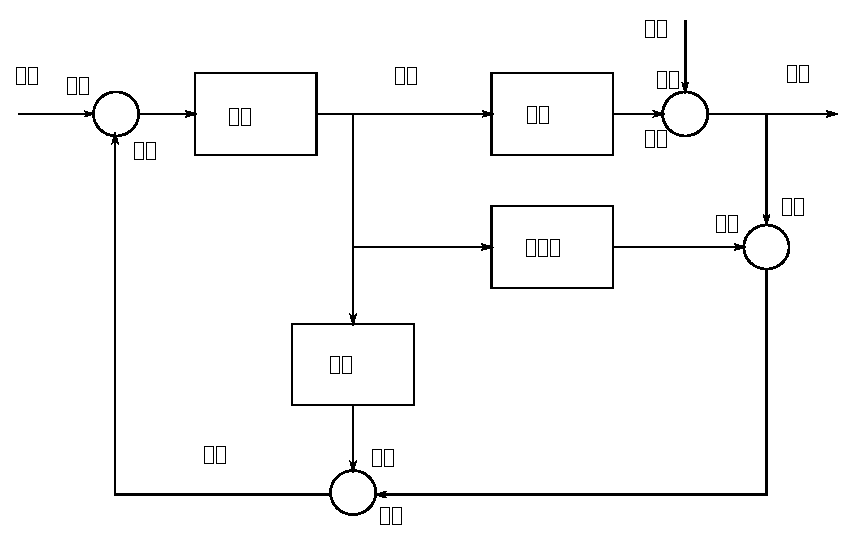
\includegraphics[scale=0.55]{pics/mimo_b3.eps}
\caption{MIMO representation of the Smith Predictor}
\label{fig:mimo_block}
\end{figure}
%For MIMO systems, the robust stability conditions are dependent on the type of perturbed model. For example, the robust conditions for MIMO systems with input multiplicative perturbations will differ for systems with output multiplicative perturbations. For a system with multiple unstructured uncertainties, the structured singular value method is typically used to prove the robust stability and robust performance of a system \cite{ZhoDoy}. 

The transfer function from the output disturbance $\vec{D}(s)$ to $\vec{Y}(s)$ is the output sensitivity function $\vec{S}(s,\rho)$, while the transfer function from $\vec{R}(s)$ to $\vec{Y}(s)$ is the complementary sensitivity function $\vec{T}(s,\rho)$:
\begin{equation}  \label{eq:sens_mimo}
\begin{split}
\vec{S}(s,\rho)&=[\vec{I}+\vec{H}(s)\vec{C}(s,\rho)]\vec{Z}^{-1}(s,\rho) \\ \vec{T}(s,\rho)&=\vec{P}(s) \vec{C}(s,\rho) \vec{Z}^{-1}(s,\rho) 
\end{split}
\end{equation}
where $\vec{Z}(s,\rho)=[\vec{I}+\vec{L}(s,\rho)]$. The objective is to determine the controller $\vec{C}(s,\rho)$ that will guarantee the robust performance and robust stability of the closed-loop SP system. 
\section{Proposed method}
\label{sec:3}
It is well known that if a SISO model is described by unstructured multiplicative uncertainty, and possesses both robustness and performance weighing functions $W_1$ and $W_2$, then the necessary and sufficient condition for robust performance is given by \cite{DFT92}:
\begin{equation}
\||W_1S|+|W_2T|\|_{\infty}<1
\end{equation}
where $S$ and $T$ are the sensitivity and complementary  sensitivity functions of a SISO system, respectively. 

For the moment, assume the case when a closed-loop MIMO system is fully decoupled. Then the MIMO sensitivity and complementary sensitivity functions can essentially be treated as functions containing independent SISO subsystems. Thus it is judicious to define $\vec{W}_1(s)$ as a diagonal filter with diagonal elements $W_{1_{q}}$ and a diagonal filter $\vec{W}_2(s)$ with diagonal elements $W_{2_{q}}$ representing, respectively, the nominal performance and multiplicative uncertainty for the SISO subsystems. This rationalization leads to the following theorem:  
 
\newtheorem{theorem}{Theorem} %Use this when you're stating a theorem
\begin{theorem} 
\label{rob_per}
Let $M_{qq}(j\omega,\rho)$ represent the diagonal elements of $\vec{H}(j\omega)\vec{C}(j\omega,\rho)$ and $N_{qq}(j\omega,\rho)$ represent the diagonal elements of $\vec{P}(j\omega)\vec{C}(j\omega,\rho)$. Suppose that $\vec{S}(s,\rho)$ and $\vec{T}(s,\rho)$ in (\ref{eq:sens_mimo}) are diagonal transfer function matrices (the closed-loop system is fully decoupled). Then the linearly parameterized controller in (\ref{eq:mimo_con}) will guarantee the closed-loop stability of the system and satisfy the following robust performance criterion:
\begin{eqnarray} \label{eq:mimo_hinf}
\| |W_{1_{q}}(j\omega)S_{qq}\jo|+ |W_{2_{q}}(j\omega)T_{qq}\jo| \|_{\infty} < 1 \nonumber\\
\mbox{for }q=1,\ldots,n_o
\end{eqnarray}
if
\begin{eqnarray} \label{eq:mimo_approx}
\{|W_{1_{q}}(j\omega)[1+M_{qq}\jo]|+|W_{2_{q}}(j\omega)N_{qq}\jo|\} \nonumber\\
\times |1+L_{D_{q}}(j\omega)| -\Psi_q\jo<0 \nonumber\\
\forall \omega \: \mbox{ for }q=1,\ldots,n_o  
\end{eqnarray}
where 
$$
\Psi_q\jo=R_e\{[1+L^*_{D_{q}}(j\omega)][1+L_{qq}\jo]\}
$$
and $S_{qq}$ and $T_{qq}$ are the $q$-th diagonal elements of $\vec{S}(s,\rho)$ and $\vec{T}(s,\rho)$, respectively. $L_{D_{q}}(s)$ is the $q$-th diagonal element of a diagonal transfer function matrix $\vec{L}_D(s)$ that contains strictly proper transfer functions which do not encircle the critical point, and $L^*_{D_{q}}$ is its complex conjugate.   
\end{theorem}
\begin{proof} %This is if you have proofs
If the closed-loop MIMO system is fully decoupled, then the MIMO sensitivity and complementary sensitivity functions can be considered as systems containing independent SISO systems. 
Since the real part of a complex number is less than or equal to its magnitude, we have
\begin{eqnarray} \label{UpperBound}
Re\{[1+L^{\ast}_{D_{q}}(j\omega)][1+L_{qq}(j\omega,\rho)]\}
\nonumber\\ \leq |[1+L^{\ast}_D(j\omega)][1+L_{qq}(j\omega,\rho)]|
\end{eqnarray}
Then, by combining (\ref{UpperBound}) and (\ref{eq:mimo_approx}) (and noting that $|1+L_{D_{q}}|=|1+L^*_{D_{q}}|$), one obtains 				
\begin{eqnarray}
\big|W_{1_{q}}(1+M_{qq} \jo)\big| + \big | W_{2_{q}}N_{qq} \jo\big| \nonumber\\ - |1+L_{qq}(\jo)|<0 \nonumber\\
 \forall \omega \: \mbox{ for }q=1,\ldots,n_o
\end{eqnarray}
The above equation can be rearranged and expressed as follows:
\begin{eqnarray}\label{eq:rob_proof}
\frac{|W_{1_{q}}(1+M_{qq}\jo)| + |W_{2_{q}}N_{qq}\jo| }{|1+L_{qq}(\jo|} <1 \nonumber\\
 \forall \omega \: \mbox{ for }q=1,\ldots,n_o 
\end{eqnarray}
Since $M_{qq}$ and $N_{qq}$ are the $q-th$ diagonal elements of $\vec{H}(s)\vec{C}(s,\rho)$ and $\vec{P}(s)\vec{C}(s,\rho)$ in (\ref{eq:sens_mimo}), respectively, it can be seen that (\ref{eq:rob_proof}) leads directly to (\ref{eq:mimo_hinf}).
\end{proof}



In order to fully decouple the MIMO system, a controller must be designed such that the off-diagonal elements of the open-loop transfer function matrix are equal to zero.
%However, decoupling the MIMO system will not necessarily generate the desired single-loop responses, since it is the diagonal elements of $\vec{L}(s,\rho)$ that represent the single-loop responses of the system. 
%Thus the objective is to effectuate decoupling while simultaneously optimize the diagonal elements to achieve the desired single-loop performance. 
The proposed method will be to define a diagonal open-loop transfer function matrix $\vec{L}_D(s)$, where the diagonal elements satisfy the desired performance for single loop systems. Therefore, by minimizing the objective function $\| \vec{L}(s,\rho)-\vec{L}_D(s) \|_{2}^{2}$, a controller can be designed to simultaneously  minimize the magnitudes of the off-diagonal elements of $\vec{L}(s,\rho)$ and drive the diagonal elements to be approximately equal to $L_{D_{q}}(s)$.

However, the resulting controller will stabilize the closed-loop system only if it is fully decoupled. In practice, with a finite order controller, it is not always possible to make the off-diagonal elements of  $\vec{L}(j\omega,\rho)$ equal to zero. In this case, the generalized Nyquist stability criterion should be used to guarantee the stability of the MIMO system. According to this theorem, the eigenvalues of the open-loop transfer function (\ref{eq:oltfmimo}) should not encircle the critical point. However, these eigenvalues are non-convex functions of the linear control parameters, which complicates the design process. A possible solution to this problem is to implement the Gershgorin band theorem in order to approximate the eigenvalues of $\vec{L}(j\omega,\rho)$. The Gershgorin bands represent disks centered at the diagonal elements of a matrix that include the eigenvalues.  For the open-loop transfer matrix $\vec{L}(j\omega,\rho)$, the radius of these disks are computed by: 
\begin{equation}
r_{q}(\omega,\rho)=\sum_{p=1,p\neq q}^{n_o} |L_{qp}(j\omega,\rho)| 
\end{equation}
where $L_{qp}(j\omega,\rho)$ represents the $qp$-th element of $\vec{L}(j\omega,\rho)$. Note that $r_{q}(\omega,\rho)$ is convex with respect to the control parameter $\rho$. The closed-loop stability of the MIMO system is guaranteed if these disks do not encircle the critical point. This precondition leads to the following theorem:
%This condition can be approximated with a convex constraint as it is shown in (\cite{GKL10b}). 

\begin{theorem} 
\label{rob_stab}
Given the open loop transfer function matrix $\vec{L}\jo$, the linearly parameterized controller (\ref{eq:mimo_con}) stabilizes the closed-loop system if
\begin{eqnarray} \label{eq:gersh_con}
|r_{q}(j\omega,\rho)[1+L_{D_{q}}(j\omega)]|-\Psi_{q}(\rho,\omega)<0 \nonumber\\
\forall \omega \; \mbox{ for }q=1,\ldots,n_o
\end{eqnarray}
\end{theorem}
\begin{proof} 
%Since the real part of a complex number is less than or equal to its magnitude, we have
%\begin{eqnarray} \label{eq:r_lt_m}
%Re\{[1+L^{\ast}_{D_{q}}(j\omega)][1+L_{qq}(j\omega,\rho)]\}
%\nonumber\\ \leq |[1+L^{\ast}_D(j\omega)][1+L_{qq}(j\omega,\rho)]|
%\end{eqnarray}
By combining the constraint in (\ref{eq:gersh_con}) and (\ref{UpperBound}) (and noting that $|1+L_{D_{q}}|=|1+L^*_{D_{q}}|$), one obtains 				
\begin{eqnarray} \label{eq:gersh_stab}
|r_{q}\jo | < |1+L_{qq}\jo | \nonumber\\
 \forall \omega \: \mbox{ for }q=1,\ldots,n_o
\end{eqnarray}
The constraint in (\ref{eq:gersh_stab}) guarantees that the disk with radius $r_q\jo$ centered at $L_{qq}\jo$ does not encircle the critical point $(-1+j0)$, and thus the system remains stable for all $\omega$.%\footnote{A more general proof for unstable systems is given in \cite{GKL10b}.}.
\end{proof}

\subsection{Primary controller design}
In designing the controller $\vec{C}(s,\rho)$ for the MIMO SP, one must consider all of the possible combinations of the uncertain delay parameters $\tau_{qp}$.  Suppose that the cardinality of  $\tau_{qp}$ is $\beta_{qp}$. Then the total number of possible combinations that must be considered in the design of the controller is given by the rule of product,
\begin{align}
&\hspace{1cm} m=\prod \beta_{qp} \nonumber \\
&\forall \;\; q=1,\ldots,n_o;\;p=1,\ldots,n_i
\end{align}
If the number of uncertainties are equal for each $\tau_{qp}$ (i.e., $\beta_{qp}=\beta_{pq}=\beta\; \forall \; \{p,q\}$), then the total number of combinations will be $m=\beta^{n_o n_i}$. By combining the constraints presented in \thref{rob_per} and \thref{rob_stab}, one can define the following optimization problem for the multimodel system:
\begin{align}\label{eq:long_con}
&\hspace{2cm} \min_\rho \sum_{c=1}^{m} \sum_{k=1}^N \|\mathbf{L}_c(j\omega_k,\rho)-\mathbf{L}_{D_{c}}(j\omega_k)\|_F \nonumber\\
&\mbox{ Subject to: } \nonumber\\
&|r_{q_{c}}(j\omega_k,\rho)[1+L_{D_{q_{c}}}(j\omega_k)]|-\Psi_{q_{c}}(\rho,\omega_k)<0 \nonumber\\
&
\{|W_{1_{q_{c}}}(j\omega_k)[1+M_{qq_{c}}(j\omega_k,\rho)]|+ \nonumber \\
&|W_{2_{q_{c}}}(j\omega_k)N_{qq_{c}}(j\omega_k,\rho)|\} 
|1+L_{D_{q_{c}}}(j\omega_k)| \nonumber \\ &-\Psi_{q_{c}}(\rho,\omega_k)<0 \nonumber\\
&\mbox{for } k=1,\ldots,N;\;  q=1,\ldots,n_o; \; c=1,\ldots,m
\end{align}
where 
\begin{align*}
\Psi_{q_{c}}(j\omega_k,\rho)&=R_e\{[1+L^*_{D_{q_{c}}}(j\omega_k)][1+L_{qq_{c}}(j\omega_k,\rho)]\} \\
M_{qq_{c}}(j\omega_k,\rho)&=\sum_{z=1}^{n_o} G_{qz_{c}}(j\omega_k)(1-e^{-j\omega_k \zeta_{qz_{c}}})C_{zq_{c}}(j\omega_k,\rho) \\
N_{qq_{c}}(j\omega_k,\rho)&=\sum_{z=1}^{n_o} P_{qz_{c}}(j\omega_k)C_{zq_{c}}(j\omega_k,\rho)
\end{align*}
and $\|\cdot\|_{F}$ is the Frobenius norm. The objective function in (\ref{eq:long_con}), which is an approximation of the 2-norm,  is convex with respect to the controller parameters $\rho$. Note that the first inequality shows that the Gershgorin bands do not encircle the critical point and so the MIMO system remains stable even if it is not fully decoupled. The second inequality guarantees the robust performance for the SISO subsystems of the decoupled MIMO system. %Notice that $M_{qq_{c}}$, $N_{qq_{c}}$, and $\Psi_{q_{c}}$ represent the $c$-th models defined in \thref{rob_per}. 

%It should be noted that the number of frequency points $N$ depends on the number of optimization variables of the particular problem. A scenario approach in selecting the minimum amount of frequency points was thoroughly discussed in \cite{GKL10b}. It is worth to reiterate the result; the number of frequency points $N$ should be chosen such that
%\begin{equation} \label{eq:freq_point}
%N \geq \frac{1}{\epsilon} \left(\ln \frac{1}{\eta}+n-1+\sqrt{2(n-1) \ln\frac{1}{\eta}}\right)
%\end{equation} 
%where the \textit{violation parameter} $\epsilon \in (0,1)$ and the \textit{confidence parameter} $\eta \in (0,1)$. 

\section{Industrial Case Studies}
\label{sec:4}
The following examples will demonstrate the effectiveness of the proposed method for several industrial processes proposed in literature.
\subsection{Case 1 - SP with fixed time delays} \label{ex:1}
In \cite{GKL10b}, the proposed method was applied to a unity feedback MIMO system with fixed time delays. The plant model is represented by a $2 \times 2$ interactive chemical process which is used in industrial applications, and was defined as:
\begin{align} \label{eq:plant}
\renewcommand{\arraystretch}{2.2}
\mathbf{P}(s)&=
\begin{bmatrix}
         G_{11}(s)e^{-6s} & G_{12}(s)e^{-10s}\\
         G_{21}(s)e^{-12s} & G_{22}(s)e^{-8s}
\end{bmatrix} \nonumber \\
&=
\begin{bmatrix}
         \dfrac{10e^{-6s}}{8s+1} & \dfrac{5e^{-10s}}{30s+1}\\[1em]
         \dfrac{-8e^{-12s}}{40s+1} & \dfrac{2e^{-8s}}{10s+1}
\end{bmatrix}
\end{align}
where the time scale is defined in minutes. The elements $G_{qp}(s)$ for $q=1,2$ and $p=1,2$ represent the strictly proper delay-free transfer functions in $\mathbf{G}_n(s)$. A relative-gain-array (RGA) analysis confirms that the system is not diagonally dominant. 

Since the time delay parameters are fixed for this process, the nominal time-delayed plant model $\mathbf{P}_n(s)$ will be chosen to be equal to $\mathbf{P}(s)$. In this manner, the open loop transfer function will be $\mathbf{L}(s,\rho)=\mathbf{G}_n(s)\mathbf{C}(s,\rho)$. The performance and uncertainty filters chosen for this case will be identical to those in \cite{GKL10b},
\begin{equation}
W_{1_{q}}=0.5 \quad , \quad W_{2_{q}}=0.5\left(\frac{2s+1}{s+1}\right) \qquad q=1,2
\end{equation}
For comparative purposes, a PI MIMO controller will be designed for this process. Thus the linearly parameterized controller will posses the following matrix form:
\begin{equation}
\renewcommand{\arraystretch}{1.3}
\vec{C}(s,\rho)=
\begin{bmatrix}
[\rho_{11_{1}} \;\; \rho_{11_{2}}]\vec{\phi}^T(s) & \;\; [\rho_{12_{1}} \;\; \rho_{12_{2}}]\vec{\phi}^T(s) \\
[\rho_{21_{1}} \;\; \rho_{21_{2}}]\vec{\phi}^T(s) & \;\; [\rho_{22_{1}} \;\; \rho_{22_{2}}]\vec{\phi}^T(s)
\end{bmatrix}
\end{equation}
where $\vec{\phi}(s)=\left[1 \;\;\;\; 1/s\right]$.
Additionally, the desired diagonal open-loop transfer function $\mathbf{L}_D(s)$ will be chosen as simple integrators with time constants equal to 30 minutes (i.e., $\vec{L}_D(s)=(\sfrac{1}{30s})\vec{I}$). The optimization problem in (\ref{eq:long_con}) can now be solved by repeating the stability constraints for each $\omega_k$. 
%Since the PI MIMO controller possesses 8 optimization variables (i.e., $n=8$), and choosing $\eta=\epsilon=0.1$, the inequality in (\ref{eq:freq_point}) suggests that a minimum of $N=150$ frequency points should be selected for evaluation. 
The frequency grid will be chosen to be between $10^{-2}$ and $10$ rad/min with $N=150$ equally spaced points. The PI MIMO controller obtained from optimization is:
$$
\renewcommand{\arraystretch}{1.3}
\mathbf{C}(s)=
\begin{bmatrix}
\dfrac{0.03289s + 0.001272}{s} & \dfrac{-0.03511s - 0.00311}{s} \\[0.4em]
\dfrac{0.05056s + 0.004511}{s} & \dfrac{0.2128s + 0.006133}{s}
\end{bmatrix}
$$
Fig. \ref{fig:comp} displays the closed loop response of the system with the controller obtained in \cite{GKL10b} and with the controller obtained with the SP. It can be seen that the controller for the SP produces no overshoot and asymptotically decouples the system much faster. Note that if the time constant of the desired open-loop transfer function matrix is decreased to 5 minutes, the rise and settling time of the system response is significantly improved.  

\begin{figure*}
\centering
\psfrag{tit1}{\hspace{-0.45cm} \tiny From $x_1$}
\psfrag{tit2}{\hspace{-0.45cm} \tiny From $x_2$}
\psfrag{tit3}{\hspace{-0.45cm} \tiny From $x_1$}
\psfrag{tit4}{\hspace{-0.45cm} \tiny From $x_2$}
\psfrag{im1}{\hspace{-0.3cm} \raisebox{0.1cm}{\tiny To $y_1$}}
\psfrag{im2}{\hspace{-0.3cm} \raisebox{0.1cm}{\tiny To $y_1$}}
\psfrag{im3}{\hspace{-0.3cm} \raisebox{0.1cm}{\tiny To $y_2$}}
\psfrag{im4}{\hspace{-0.3cm} \raisebox{0.1cm}{\tiny To $y_2$}}
\psfrag{re}{\hspace{-0.7cm} \raisebox{-0.08cm}{\tiny Time (minutes)}}
\hspace*{-0.3cm}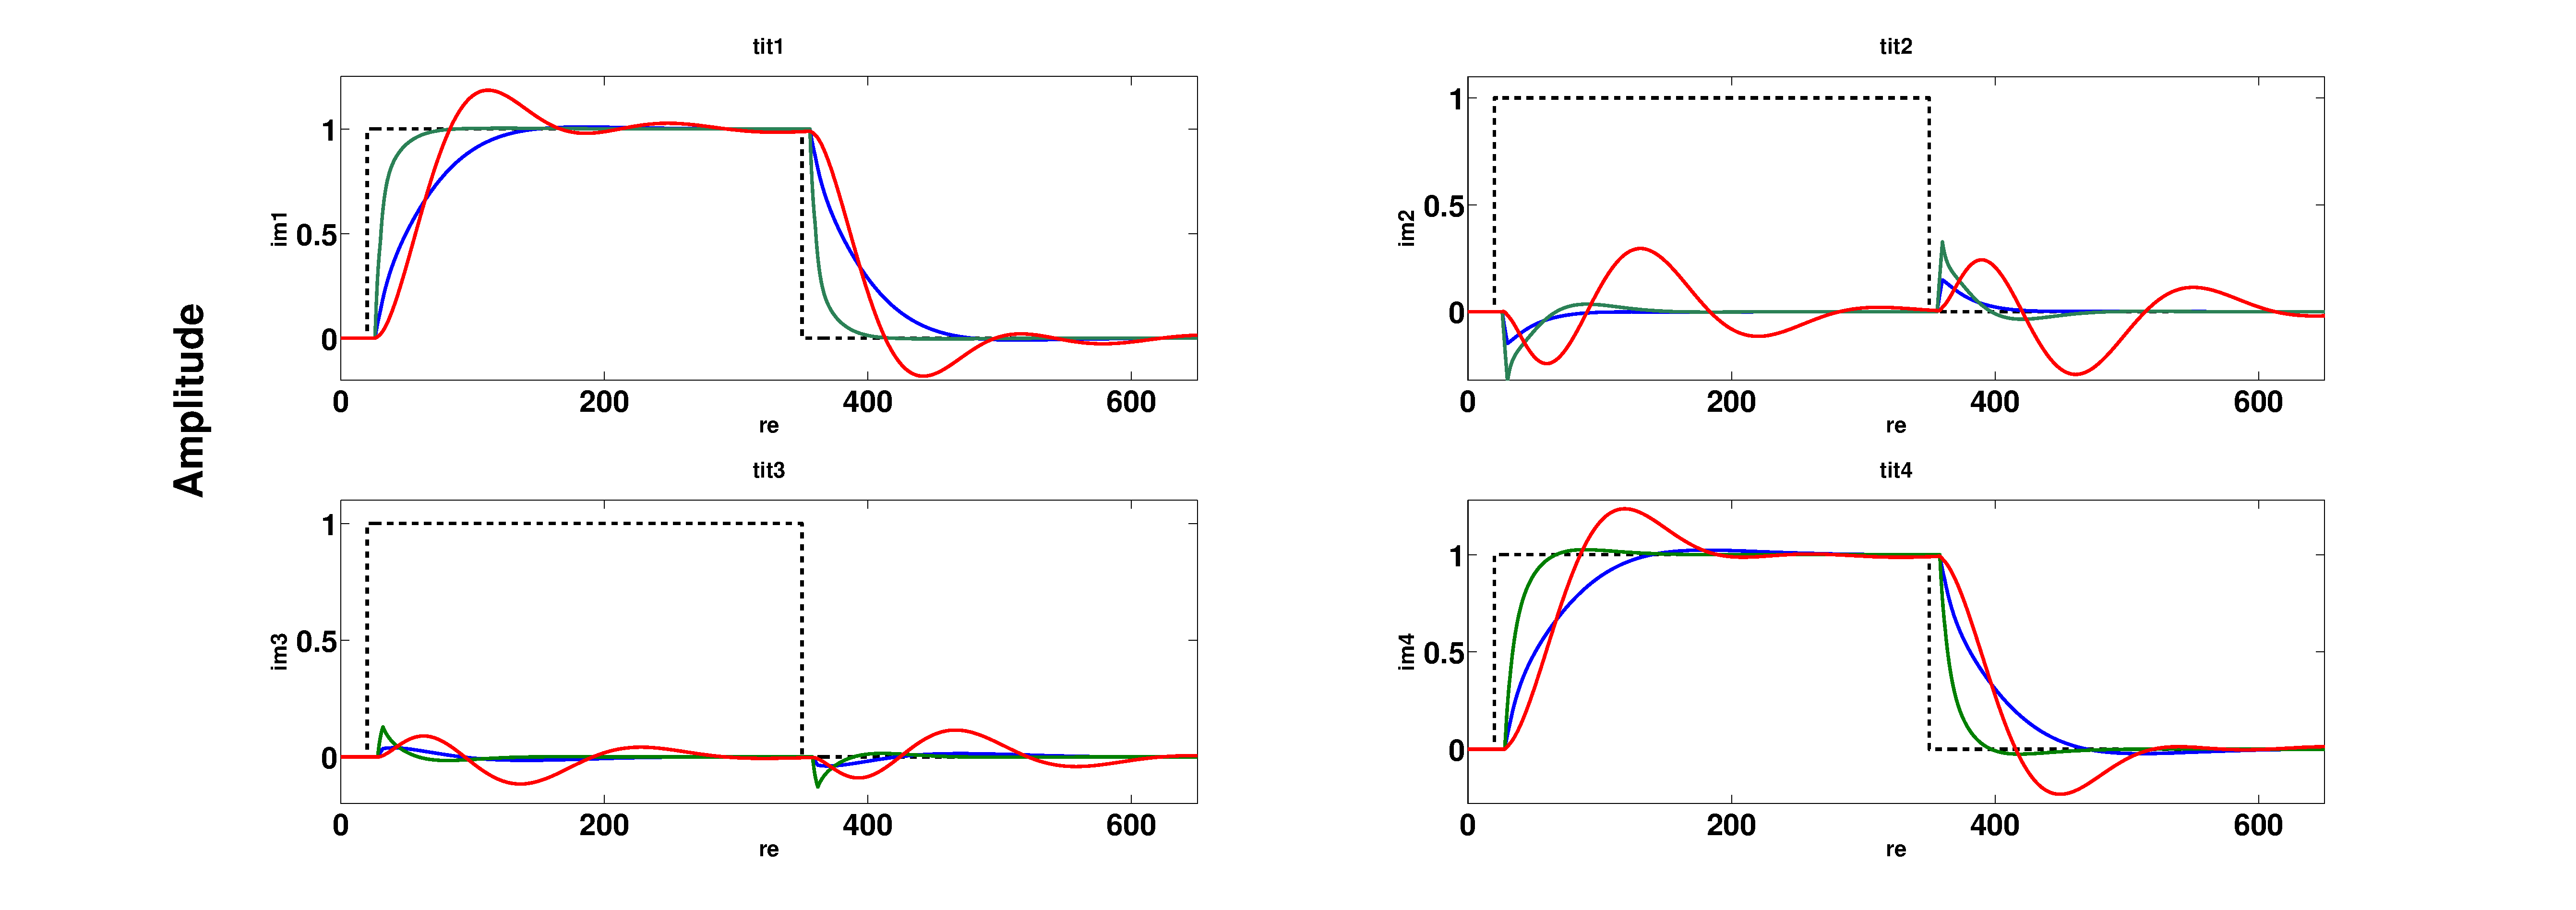
\includegraphics[width=0.85\textwidth]{pics/comp_ld_2.eps}
\caption{Closed loop comparison between time delayed MIMO system with unity feedback and time delayed MIMO SP: unit step reference signal (black, dash), response with system proposed in \cite{GKL10b} (red, solid), response with SP and with $diag \left(\mathbf{L}_D(s)\right)=\frac{1}{30s}$ (blue, solid), response with SP and with $diag \left(\mathbf{L}_D(s)\right)=\frac{1}{5s}$ (green, solid).}
\label{fig:comp}
\end{figure*}



\subsection{Case 2 - SP with uncertain time delays} \label{ex:2}
The proposed optimization problem will now be applied to an uncertain time-delayed MIMO SP. Consider the $2 \times 2$ plant process $\mathbf{P}(s)$ ($\mbox{i.e., }c=1$) that was analyzed in Case (1). The time delays for this plant will now possess uncertain values that will belong to a set. This plant will now be represented as follows:
\begin{equation}\label{eq:uncert_plant}
\renewcommand{\arraystretch}{2.2}
\vec{P}(s)=
\begin{bmatrix}
         \dfrac{10e^{-\tau_{11}s}}{8s+1} & \dfrac{5e^{-\tau_{12}s}}{30s+1}\\[0.6em]
         \dfrac{-8e^{-\tau_{21}s}}{40s+1} & \dfrac{2e^{-\tau_{22}s}}{10s+1}
\end{bmatrix}
\end{equation}
where the time delays $\tau_{qp}$ possess values in the sets:
\begin{equation}\label{eq:mimo_un}
\tau_{11}=\{3,9\} \quad \tau_{12}=\{7,13\} \quad
\tau_{21}=\{9,15\} \quad \tau_{22}=\{5,11\}
\end{equation}
The nominal model  is the same as defined in (\ref{eq:plant}).
%\begin{align}
%\renewcommand{\arraystretch}{2.2}
%\vec{P}_n(s)&=
%\begin{bmatrix}
%         G_{11}(s)e^{-6s} & G_{12}(s)e^{-10s}\\
%         G_{21}(s)e^{-12s} & G_{22}(s)e^{-8s}
%\end{bmatrix} \nonumber\\
%&=
%\begin{bmatrix}
%         \frac{10e^{-6s}}{8s+1} & \frac{5e^{-10s}}{30s+1}\\[1em]
%         \frac{-8e^{-12s}}{40s+1} & \frac{2e^{-8s}}{10s+1}
%\end{bmatrix}
%\end{align}
Again, the elements $G_{qp}(s)$ for $q=1,2$ and $p=1,2$ represent the strictly proper delay-free transfer functions in $\vec{G}_n(s)$. The performance and uncertainty filters chosen for this example will be identical to those in section (\ref{ex:1}). The desired diagonal open-loop transfer function $\vec{L}_D(s)$ will be chosen as simple integrators with time constants equal to 7 minutes (i.e., $\vec{L}_D(s)=(\sfrac{1}{7s})\vec{I}$). 

%Comment out RGA analysis
\iffalse
In order to observe the interactions of this process, the relative gain array (RGA), defined as $\Lambda[\Gamma]=\Gamma\ast (\Gamma^{-1})^T$ (where the symbol $\ast$ denotes element wise multiplication), can be used to analyze the coupling affects between each pairing of the elements in $\vec{P}_n(s)$. The frequency dependent RGA of $\vec{P}_n(s)$ is shown in Fig. \ref{fig:RGA}. 
\begin{figure}[H]
\centering
\psfrag{omega}{\hspace{-0.4cm} \raisebox{-0.2cm}{\scriptsize $\omega \; \left[\frac{rad}{min}\right]$}}
\psfrag{RGA}{\hspace{-0.7cm} \scriptsize $\Lambda [\vec{P}_n(j\omega)]$}
\centerline{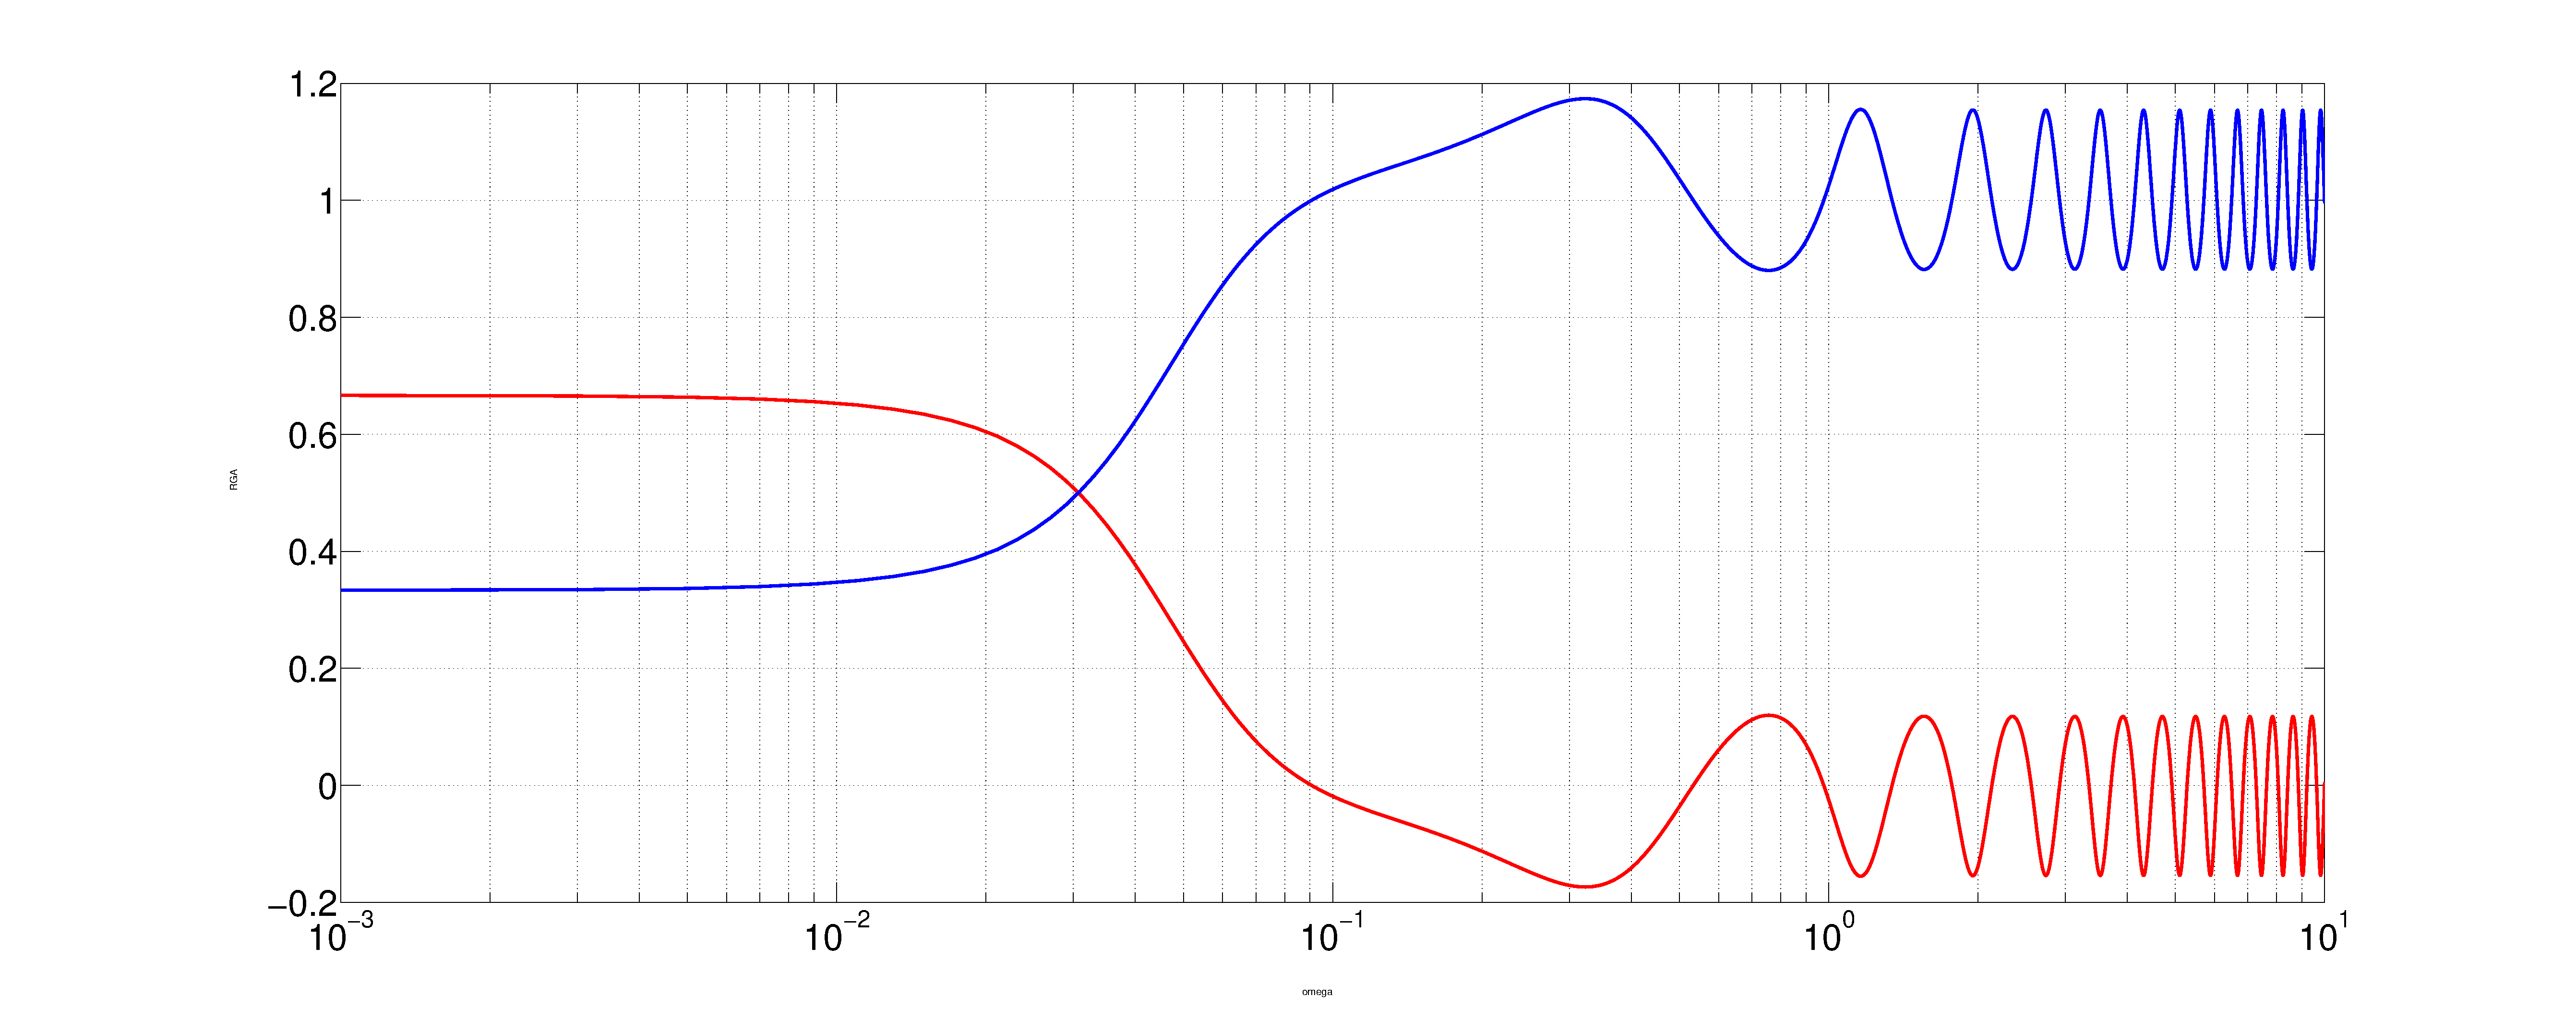
\includegraphics[scale=0.11]{pics/RG.eps}}
\caption{RGA plot of $\vec{P}_n(s)$: diagonal elements of $\Lambda [\vec{P}_n(j\omega)]$ (blue, solid), off diagonal elements of $\Lambda [\vec{P}_n(j\omega)]$ (red, solid).}
\label{fig:RGA}
\end{figure}
The most severe interaction occurs when $\Lambda_{qp}=0.5$ for $q=1,2$ and $p=1,2$. This can be seen in Fig. \ref{fig:RGA} as the intersecting point of  all functions $\Lambda_{qp}$, which occurs at a frequency of approximately  0.0307 rad/min.
Consider the case when $s=0$ (steady state response to a step input). The RGA matrix for this case will be: 
\begin{equation}
\Lambda[\vec{P}_n(s)]\Big|_{s=0}=
\begin{bmatrix}
0.3333 & 0.6667 \\ 0.6667 & 0.3333
\end{bmatrix}
\end{equation}
Since $0< \Lambda_{qp} < 1$ for $p,q=1,2$, interactions do exist, and the system is coupled. The permuted identity matrix can also be computed as follows:
\begin{equation}
\lim_{k \to \infty} \Lambda^k[\vec{P}_n(s)]\Big|_{s=0} = \begin{bmatrix}
0.5 & 0.5\\0.5 & 0.5
\end{bmatrix}
\end{equation}
which confirms that the plant process is not diagonally dominant at steady state. 
\fi

For simplicity, a PI controller will be designed for this process. Note that in designing this controller, all possible combinations of the uncertainties in (\ref{eq:mimo_un}) must be considered. Therefore, since $\beta_{qp}=2 \; \forall \; \{p,q\}$, there will be a total of $m=2^4$ possible cases to consider. The optimization problem in (\ref{eq:long_con}) can now be solved by repeating the stability constraints for each combination of the uncertainties in (\ref{eq:mimo_un}). The frequency grid will be chosen to be between $10^{-2}$ and $10$ rad/min with $N=150$ equally spaced points. The PI MIMO controller obtained from the optimization problem is:
$$
\renewcommand{\arraystretch}{1.3}
\vec{C}(s)=
\begin{bmatrix}
\dfrac{0.06234s + 0.001464}{s} & \dfrac{-0.04803s - 0.005408}{s} \\[0.4em]
\dfrac{0.1585s + 0.0168}{s} & \dfrac{0.3113s + 0.005995}{s}
\end{bmatrix}
$$
Fig. \ref{fig:mimo1} displays the closed-loop MIMO response to a step input. Notice that with this controller, the MIMO process achieves robust performance while simultaneously decoupling the system. The Gershgorin bands are depicted in Fig. \ref{fig:mimo2} for the system possessing the largest delay time uncertainty ($\tau_{11}=9$, $\tau_{12}=13$, $\tau_{21}=15$, $\tau_{22}=11$). The red and blue bands possess a radius of $|r_{q}(j\omega_k)|$ for $q=1,2$ and $k=1,\ldots,N$. 
\begin{figure*}
\centering
\psfrag{tit1}{\hspace{-0.45cm} \tiny From $x_1$}
\psfrag{tit2}{\hspace{-0.45cm} \tiny From $x_2$}
\psfrag{tit3}{\hspace{-0.45cm} \tiny From $x_1$}
\psfrag{tit4}{\hspace{-0.45cm} \tiny From $x_2$}
\psfrag{im1}{\hspace{-0.3cm} \raisebox{0.1cm}{\tiny To $y_1$}}
\psfrag{im2}{\hspace{-0.3cm} \raisebox{0.1cm}{\tiny To $y_1$}}
\psfrag{im3}{\hspace{-0.3cm} \raisebox{0.1cm}{\tiny To $y_2$}}
\psfrag{im4}{\hspace{-0.3cm} \raisebox{0.1cm}{\tiny To $y_2$}}
\psfrag{re}{\hspace{-0.7cm} \raisebox{-0.05cm}{\tiny Time (minutes)}}
\centerline{\includegraphics[width=0.85\textwidth]{pics/test.eps}}
\caption{MIMO response to a unit step input: reference signal (black,dash), the remaining $\Omega=16$ closed-loop responses are for all possible combinations of the time delay parameters in (\ref{eq:mimo_un}).}
\label{fig:mimo1}
\end{figure*}
Notice how the Gershgorin bands never intersect with the performance filter centered at $(-1+j0)$. This proves that the MIMO system is stable, robust, and satisfies the optimization criterion in (\ref{eq:long_con}).
%\vspace{0.7cm}
\begin{figure}
%\vspace{-0.7cm}
\centering
\psfrag{R}{\hspace{-0.5cm} \raisebox{-0.15cm}{\small $\Re_e \{Z(j\omega) \}$}}
\psfrag{Y}{\hspace{-0.7cm} \small $\Im_m \{Z(j\omega) \}$}
\hspace*{-0.3cm}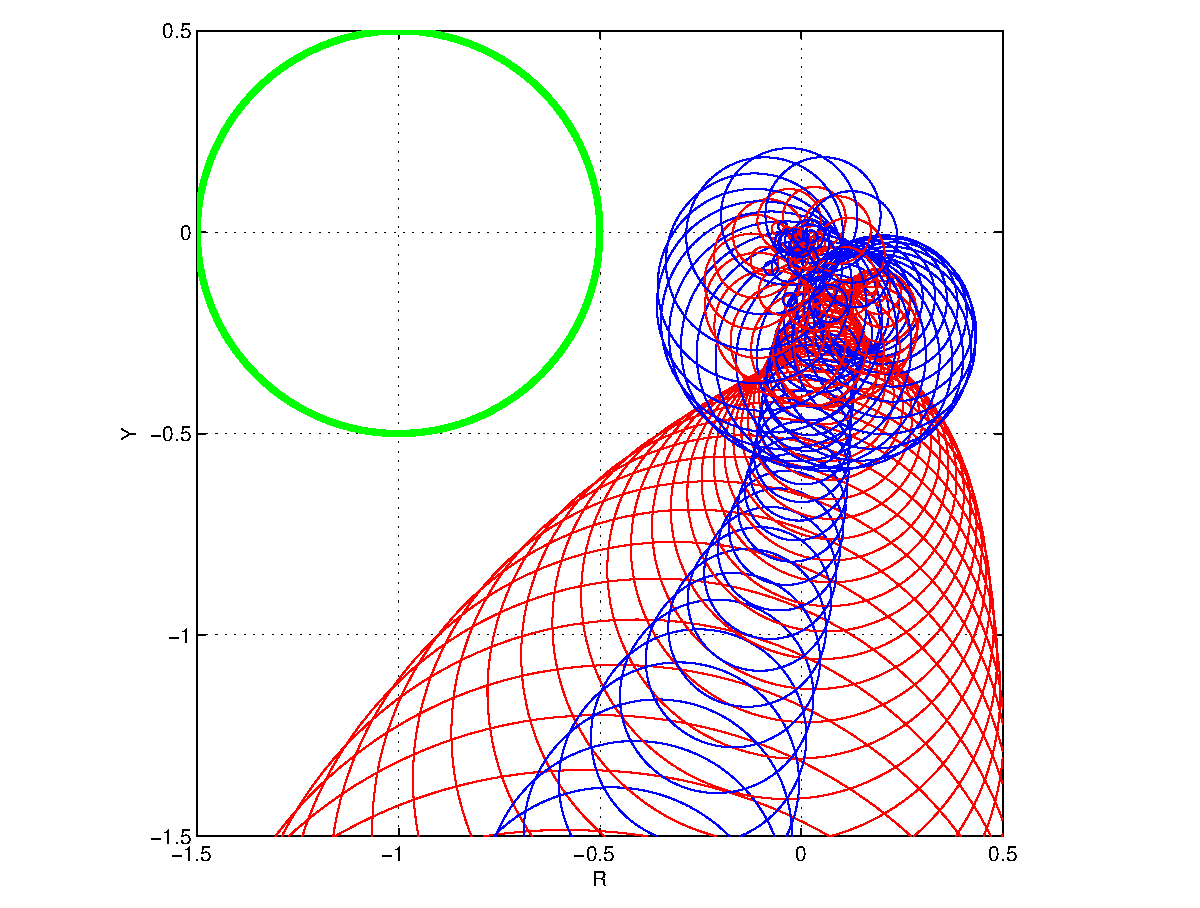
\includegraphics[scale=0.5]{pics/gersh.eps}
\caption{Gershgorin bands centered at $L_{qq}$ with the largest time delay combination in (\ref{eq:mimo_un}): performance filter with $|W_{1_{q}}|=0.5$ (green circle), Gershgorin bands corresponding to $q=1$ (blue circles), Gershgorin bands corresponding to $q=2$ (red circles). Note that $Z(j\omega)$ is simply the complex number representation of each circle in the plot.}
\label{fig:mimo2}
\end{figure}
 

\subsection{Case 3 - The Shell control problem} \label{ex:3}
The multivariable heavy oil fractionator (known as the Shell process) is a highly coupled system which is predominantly used in petrochemical processes. Efficient control methods are essential for attaining viable production rates, minimizing energy consumption, and reducing the overall operating costs. These types of systems are difficult to control for two reasons: the system interactions are strong, and the large time delays that are inherent to the system dynamics. 

Consider the $2 \times 3$ industrial Shell problem in \cite{RC06}, 
\begin{align}\label{eq:shell_nom}
\renewcommand{\arraystretch}{2.2}
\vec{P}_n(s)&=
\begin{bmatrix}
         G_{11}(s)e^{-81s} & G_{12}(s)e^{-84s} & G_{13}(s)e^{-81s}\\
         G_{21}(s)e^{-54s} & G_{22}(s)e^{-42s} & G_{32}(s)e^{-45s}
\end{bmatrix} \nonumber\\
&=
\begin{bmatrix}
         \dfrac{4.05e^{-81s}}{50s+1} & \dfrac{1.77e^{-84s}}{60s+1} & \dfrac{5.88e^{-81s}}{50s+1}\\[1em]
         \dfrac{5.39e^{-54s}}{50s+1} & \dfrac{5.72e^{-42s}}{60s+1} & \dfrac{6.9e^{-45s}}{40s+1}
\end{bmatrix}
\end{align}
where the time scale is defined in minutes. Note that (\ref{eq:shell_nom}) is represented as the nominal model of the process. 
It should be noted that the controller outputs $[u_1(t) \; u_2(t) \; u_3(t)]^T$ should be within the saturation bounds of the physical system : $[-0.5 \, , \, 0.5]$ (see \cite{VWG02}). 
The elements $G_{qp}(s)$ for $q=1,2$ and $p=1,2,3$ represent the strictly proper delay-free transfer functions in $\vec{G}_n(s)$. Now consider the case when the time delays are varied to $+20\%$ of their nominal values shown in (\ref{eq:shell_nom}). As with the previous example, the plant $\vec{P}(s)$ can be represented as a system with uncertain time delays. Since $\beta_{qp}=2 \; \forall \; \{p,q\}$, there will be a total of $m=2^6=64$ possible cases to consider.%\footnote{Note that the nominal time delays are also being considered in the controller design process, since it is desired that the controller remains robust for all combinations of perturbed time delays.}. 

For comparative purposes, a PI controller will be designed for this process. Thus the controller $\vec{C}(s,\rho)$ will be a $3 \times 2$ transfer function matrix with $n=12$ optimization parameters $\rho$. 
%By selecting $\eta=\epsilon=0.1$, the inequality in (\ref{eq:freq_point}) suggests that a minimum of $N=205$ frequency points should be selected for evaluation. 
The frequency grid will be chosen to be between $10^{-4}$ and $10$ rad/min with $N=200$ equally spaced points (since the frequencies of interest of the open-loop system lie within this range). The desired diagonal open-loop transfer function matrix will be chosen as simple integrators with bandwidths that are approximately $20\%$ greater than the open-loop system bandwidths (i.e., $\vec{L}_D(s)=(\sfrac{1}{35s})\vec{I}$). By solving the optimization problem in (\ref{eq:long_con}) for each combination of the uncertainties (i.e., $\{\tau_{11},\ldots,\tau_{qp}\} \; \forall \; \{p,q\}$ where $\tau_{qp} \in \{\zeta_{qp},1.2\zeta_{qp}\} $), one obtains the following PI controller
$$
\renewcommand{\arraystretch}{1.3}
\vec{C}(s)=
\begin{bmatrix}
\dfrac{0.2053s + 0.004997}{s} & \dfrac{-0.01315s - 0.00146}{s} \\[0.4em]
\dfrac{-0.6735s - 0.01008}{s} & \dfrac{0.4977s + 0.008098}{s} \\[0.4em]
\dfrac{0.2839s + 0.004451}{s} & \dfrac{-0.1041s - 0.001432}{s}
\end{bmatrix}
$$
Fig. \ref{fig:shell_no_del} displays the closed-loop step response of the SP for the nominal delay case, while Fig. \ref{fig:shell_del} displays the response with the worst case delay (the case where $\tau_{qp}=1.2\zeta_{qp} \; \forall \; \{p,q\}$). 


\begin{figure*}[]
\centering
\psfrag{tit1}{\hspace{-0.45cm} \scriptsize From $x_1$}
\psfrag{tit2}{\hspace{-0.45cm} \scriptsize From $x_2$}
\psfrag{tit3}{\hspace{-0.45cm} \scriptsize From $x_1$}
\psfrag{tit4}{\hspace{-0.45cm} \scriptsize From $x_2$}
\psfrag{im1}{\hspace{-0.3cm} \raisebox{0.1cm}{\scriptsize To $y_1$}}
\psfrag{im2}{\hspace{-0.3cm} \raisebox{0.1cm}{\scriptsize To $y_1$}}
\psfrag{im3}{\hspace{-0.3cm} \raisebox{0.1cm}{\scriptsize To $y_2$}}
\psfrag{im4}{\hspace{-0.3cm} \raisebox{0.1cm}{\scriptsize To $y_2$}}
\psfrag{re}{\hspace{-0.7cm} \raisebox{-0.05cm}{\scriptsize Time (minutes)}}
\centerline{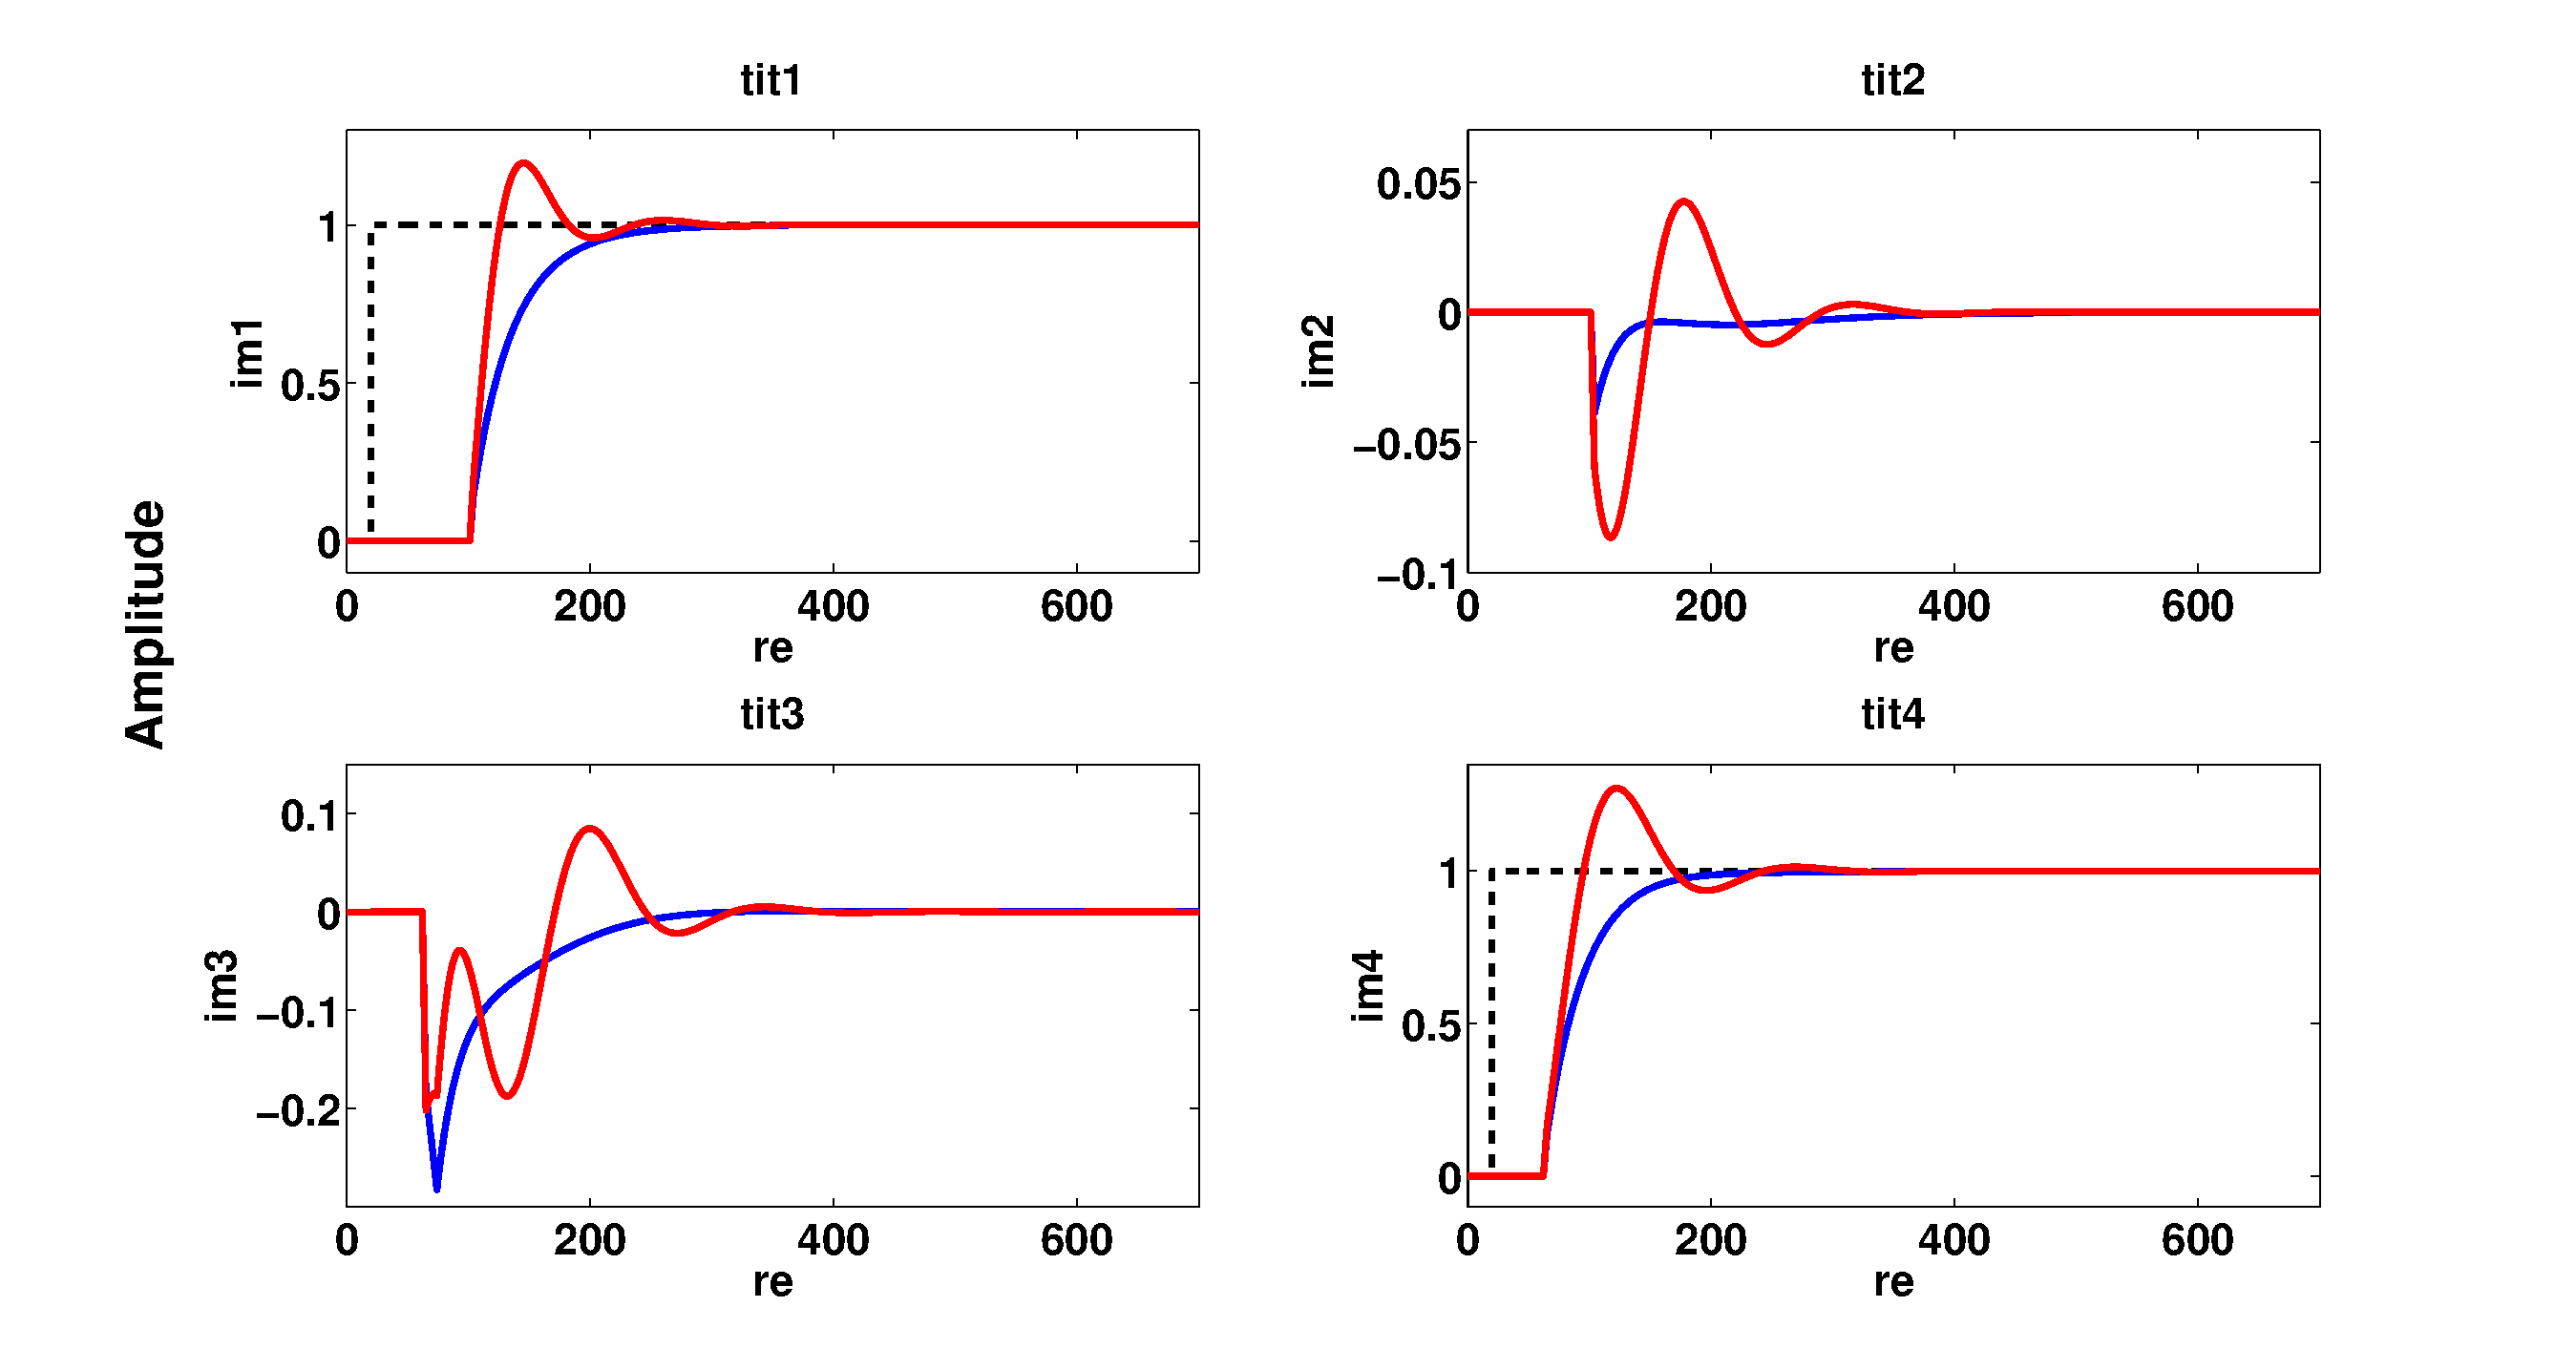
\includegraphics[width=0.7\textwidth]{pics/Rob_comp_LD35_1.eps}}
\caption{MIMO SP closed-loop response to a unit step input with $\tau_{qp}=\zeta_{qp} \; \forall \; \{p,q\}$: reference signal (black,dash), output response with the proposed optimization method (blue, solid), output response with the proposed method in \cite{RC06} (red, solid), which is based on the ``squared down" method.}
\label{fig:shell_no_del}
\end{figure*}

\begin{figure*}[]
\centering
\psfrag{tit1}{\hspace{-0.45cm} \scriptsize From $x_1$}
\psfrag{tit2}{\hspace{-0.45cm} \scriptsize From $x_2$}
\psfrag{tit3}{\hspace{-0.45cm} \scriptsize From $x_1$}
\psfrag{tit4}{\hspace{-0.45cm} \scriptsize From $x_2$}
\psfrag{im1}{\hspace{-0.3cm} \raisebox{0.1cm}{\scriptsize To $y_1$}}
\psfrag{im2}{\hspace{-0.3cm} \raisebox{0.1cm}{\scriptsize To $y_1$}}
\psfrag{im3}{\hspace{-0.3cm} \raisebox{0.1cm}{\scriptsize To $y_2$}}
\psfrag{im4}{\hspace{-0.3cm} \raisebox{0.1cm}{\scriptsize To $y_2$}}
\psfrag{re}{\hspace{-0.7cm} \raisebox{-0.05cm}{\scriptsize Time (minutes)}}
\centerline{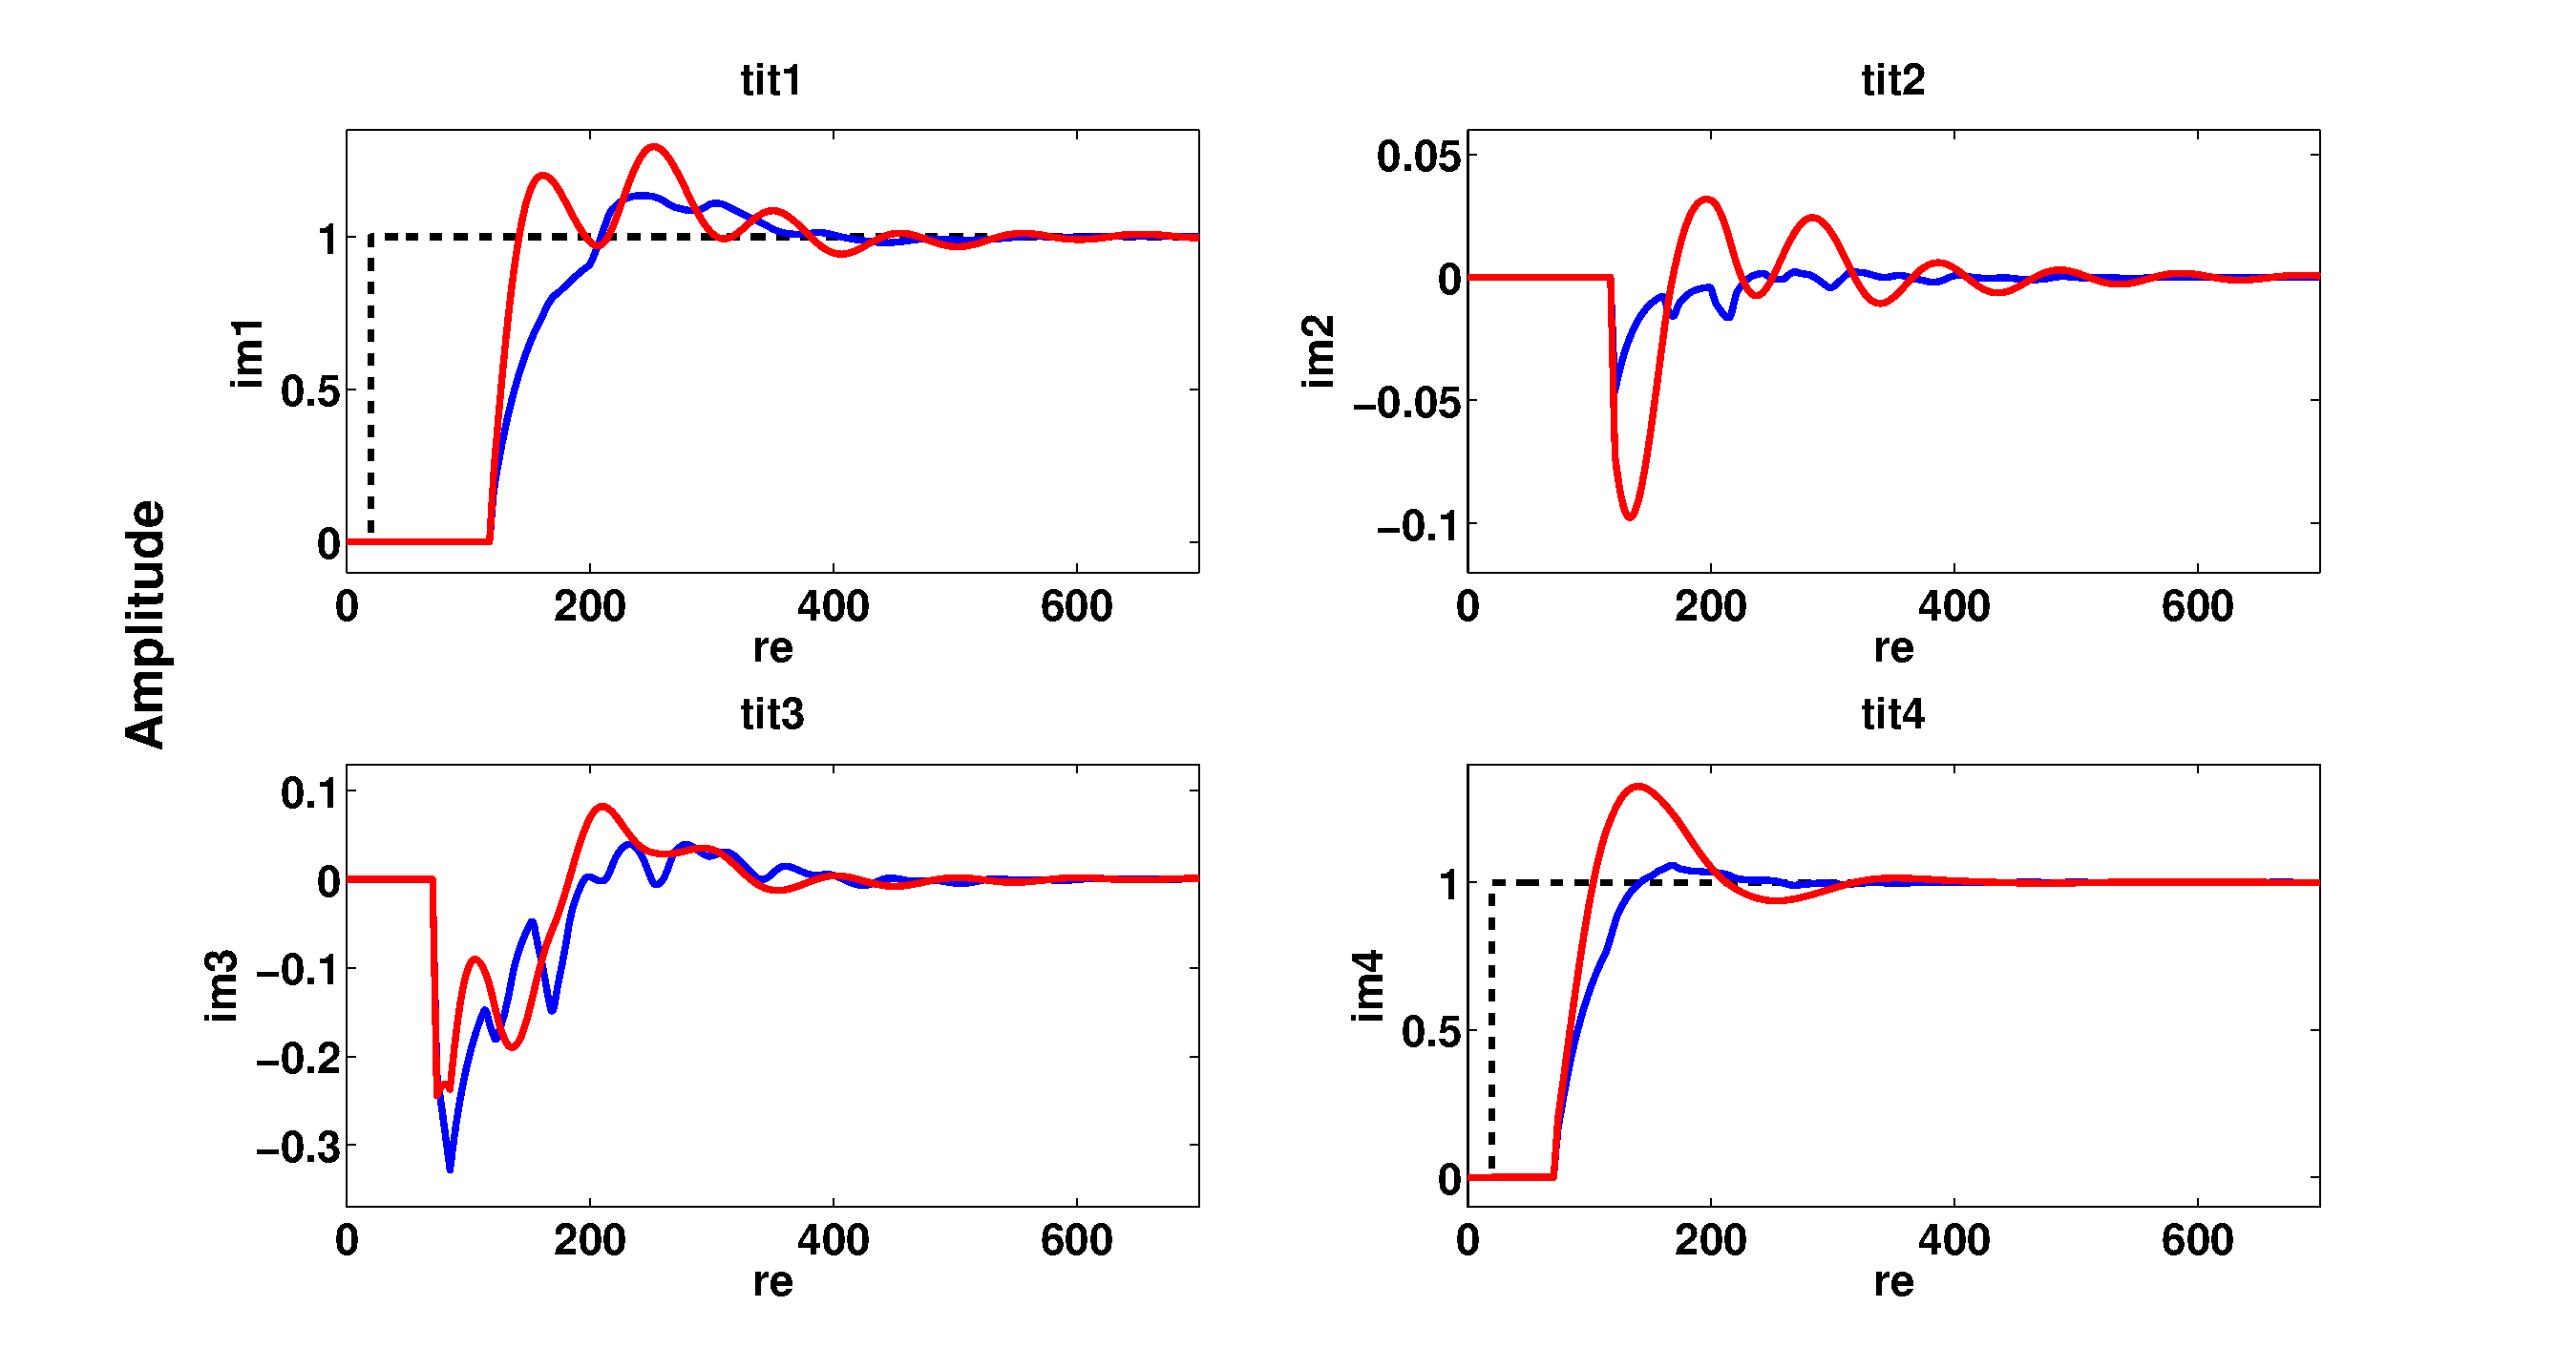
\includegraphics[width=0.7\textwidth]{pics/Rob_comp_LD35_2.eps}}
\caption{MIMO SP closed-loop response to a unit step input with $\tau_{qp}=1.2\zeta_{qp} \; \forall \; \{p,q\}$: reference signal (black,dash), output response with the proposed optimization method (blue, solid), output response with the proposed method in \cite{RC06} (red, solid), which is based on the ``squared down" method.}
\label{fig:shell_del}
\end{figure*}
From Fig. \ref{fig:shell_no_del} and Fig. \ref{fig:shell_del}, it can be observed that the purposed method in this paper produces improved SISO subsystem performance with minimal overshoot. In addition, the decoupling transients are significantly reduced for both the nominal and worst case output responses. Fig. \ref{fig:shell_in} displays the controller outputs of the system. 
\begin{figure*}[]
\centering
\psfrag{im1}{\hspace{-0.3cm} \raisebox{0.1cm}{\scriptsize$u_1(t)$}}
\psfrag{im2}{\hspace{-0.3cm} \raisebox{0.1cm}{\scriptsize$u_2(t)$}}
\psfrag{im3}{\hspace{-0.3cm} \raisebox{0.1cm}{\scriptsize$u_3(t)$}}
\psfrag{re}{\hspace{-0.7cm} \raisebox{-0.2cm}{\tiny Time (minutes)}}
\centerline{\includegraphics[width=0.9\textwidth]{pics/Rob_comp_LD35_in2.eps}}
\caption{MIMO SP controller output response to a unit step reference: Controller output response of proposed method with $\tau_{qp}=\zeta_{qp}$ (blue, solid), controller output response of ``squared down" method in \cite{RC06} with $\tau_{qp}=\zeta_{qp}$ (red, solid), controller output response of proposed method with $\tau_{qp}=1.2\zeta_{qp}$ (blue, dash), controller output response of ``squared down" method in \cite{RC06} with $\tau_{qp}=1.2\zeta_{qp}$ (red, dash)}
\label{fig:shell_in}
\end{figure*}

\section{Conclusion}
\label{sec:5}
This paper has proposed a new method for computing multivariable SP controllers with $H_\infty$ performance. The method is based on a convex approximation of the $H_\infty$ robust performance criterion in the Nyquist diagram. This approximation relies on the choice of a desired open-loop transfer function $\vec{L}_D$ for the dead-time free model of the plant. With a linearly parameterized controller, one possesses the flexibility to design PI, PID, or higher order controllers for a system. For the industrial processes considered in this paper, the proposed method has been proven to be robust; $H_{\infty}$ performance was achieved for MIMO systems with both multiplicative and time delay uncertainties. The solution to the optimization problem generates a controller such that a system becomes decoupled and simultaneously optimizes the single-loop performances of the SISO subsystems.

%The controller design examples illustrated in this paper considered a finite amount of discrete values to represent the uncertainties in the time delays. However, the proposed optimization methods can be applied for a system(s) with $\alpha$ number of uncertainties within a specified range, where $\{\exists\alpha \in \mathbb{Z}^+ | \; 0<\alpha<\infty \} $.


%\appendix[Proof of Equations] %Put your appendix here
\iffalse

%\section*{Acknowledgment}
%\addcontentsline{toc}{section}{Acknowledgment}
%Your acknowledgments go here.
\begin{thebibliography}{99.}%
% and use \bibitem to create references.
%
% Use the following syntax and markup for your references if
% the subject of your book is from the field
% "Mathematics, Physics, Statistics, Computer Science"
%
% Contribution
%\bibitem{Bro79} C. B. Brosilow. The structure and design of Smith
%predictors from the viewpoint of inferential control.
%In Proceedings of Joint American Control Conference,
%Denver, Colorado, 1979.
%
\bibitem{VK13} V. De Oliveira, A. Karimi. Robust Smith predictor design for time-delay systems with $H_\infty$ performance.  IFAC Joint Conference, Grenoble, France, February 4-6, 2013.
%
%\bibitem{Dep85} A. M. De Paor. A modified Smith predictor and controlled
%for unstable processes with time delay. International
%Journal of Control, 41(4):1025–1036, 1985.
%
\bibitem{DFT92} C. J. Doyle, B. A. Francis, and A. R. Tannenbaum.
Feedback Control Theory. Mc Millan, New York, 1992.
%
\bibitem{GKL10a} G. Galdos, A. Karimi, and R. Longchamp. Robust controller
design by convex optimization based on finite
frequency samples of spectral models. In 49th IEEE
Conference on Decision and Control, Atlanta, USA,
2010a.
%
\bibitem{GKL10b} G. Galdos, A. Karimi, and R. Longchamp. $H_{\infty}$ controller
design for spectral MIMO models by convex optimization.
Journal of Process Control, 20(10):1175 – 1182,
2010b.
%
%\bibitem{Hag92} T. Hagglund. A predictive PI controller for processes with
%long dead times. IEEE Control Systems Magazine, 12
%(1):57–60, 1992.
%
%\bibitem{HWC95} C. C. Hang, Q. Wang, and L. S. Cao. Self-tuning Smith
%predictors for processes with long dead time. International
%journal of adaptive control and signal processing,
%9(3):255–270, 1995.
%
%\bibitem{KG10} A. Karimi and G. Galdos. Fixed-order H∞ controller design
%for nonparametric models by convex optimization.
%Automatica, 46(8):1388–1394, 2010.
%
%\bibitem{Kay01} I. Kaya. Tuning Smith predictors using simple formulas
%derived from optimal responses. Industrial and engineering
%chemistry research, 40(12):2654–2659, 2001.
%
\bibitem{LHW08} C. Lai, P. Hsu, and B. Wang. Design of the adaptive Smith predictor for the time-varying network control system. SICE Annual Conference, The University Electro-Communications, Japan, p. 2933 - 2938, 2008.
%
%\bibitem{LLSL99} D. Lee, M. Lee, S. Sung, and I. Lee. Robust PID tuning
%for Smith predictor in the presence of model uncertainty.
%Journal of Process Control, 9(1):79–85, 1999.
%
%\bibitem{LCGZ05} T. Liu, Y. Z. Cai, D. Y. Gu, and W. D. Zhang. New
%modified Smith predictor scheme for integrating and
%unstable processes with time delay. IEE Proceedings-
%Control Theory and Applications, 152(2):238–246, 2005.
%
%\bibitem{MA98} S. Majhi and D. P. Atherton. A new Smith predictor and
%controller for unstable and integrating processes with
%time delay. In Proceedings of the 37th IEEE Conference
%on Decision and Control, pages 1341–1345, 1998.
%
\bibitem{MZ00} G. Meinsma and H. Zwart. On H∞ control for dead-time
systems. IEEE Transactions on Automatic Control, 45
(2):272–285, 2000.
%
\bibitem{Mir03} L. Mirkin. On the extraction of dead-time controllers
and estimators from delay-free parametrizations. IEEE
Transactions on Automatic Control, 48(4):543–553,
2003.
%
\bibitem{NC00} J. E. Normey-Rico and E. F. Camacho. Multivariable generalised predictive controller based on the Smith predictor. IEEE Proceedings in Control Theory Applications, Vol. 147, No. 5, 2000.
%
\bibitem{NC07} J. E. Normey-Rico and E. F. Camacho. Control of deadtime
processes. Springer Verlag, 2007.
%
%\bibitem{NC09} J. E. Normey-Rico and E. F. Camacho. Unified approach
%for robust dead-time compensator design. Journal of
P%rocess Control, 19(1):38–47, 2009.
%
%\bibitem{Pal80} Z. J. Palmor. Stability properties of Smith dead-time compensator
%controllers. International Journal of Control,
32:937–49, 1980.
%
%\bibitem{Pal96} Z. J. Palmor. Time-delay compensation Smith predictor
%and its modifications. In W. Levine, editor, The Control
%Handbook. CRC Press, Boca Raton, FL, 1996.
%
%\bibitem{PB94} Z. J. Palmor and M. Blau. An auto-tuner for Smith dead
%time compensator. International Journal of Control, 60
%(1):117–135, 1994.
%
\bibitem{SBP09} R. S. Sanchez-Pena, Y. Bolea and V. Puig. MIMO Smith predictor: Global and structured robust performance analysis. Journal of Process Control 19:163-177, 2009.
%
%\bibitem{SS93} C. Santacesaria and R. Scattolini. Easy tuning of Smith
%predictor in presence of delay uncertainty. Automatica,
%29(6):1595–1597, 1993.
%
\bibitem{Sko} S. Skogestad and I. Postlethwaite. Multivariable Feedback Control; Analysis and Design. John Wiley and Sons, England, 1996.
%
\bibitem{Smi57} O. J. M. Smith. Closer control of loops with dead time.
Chemical Engineering Progress, 53(5):217–219, 1957.
%
\bibitem{ZL06} W. Zhang and C. Lin. Multivariable Smith Predictors Design for Nonsquare Plants. IEEE Transactions on Control Systems Technology,
Vol. 14, No. 6, 2006.
%
\bibitem{Zho03a} Q. C. Zhong. On standard H∞ control of processes with a single delay. IEEE Transactions on Automatic Control,
48(6):1097–1103, 2003.
%
%\bibitem{ZhoDoy} K. Zhou and J. Doyle. Essentials of Robust Control. Prentice-Hall, Upper Saddle River, New Jersey, USA, 1998.
%
\bigskip


\end{thebibliography}
\fi

%\begin{IEEEbiographynophoto}
%Author1 Biography
%\end{IEEEbiographynophoto}
%\smallskip{}
%\begin{IEEEbiographynophoto}
%Author2 Biography
%\end{IEEEbiographynophoto}

\bibliography{linear}

\end{document}
